\documentclass[english]{article}
\usepackage[utf8]{inputenc}
\usepackage[T1]{fontenc}
\usepackage{babel}
\usepackage{amsmath, amssymb}
\usepackage{graphicx}
\usepackage[dvipsnames]{xcolor}
\usepackage{multirow}
\usepackage{fancyhdr}
\newcommand{\scidatalogo}{
\includegraphics[height=36pt]{SciData_logo.jpg}}
\newcommand{\overleaflogo}{
\includegraphics[height=36pt]{Overleaf-logo-300dpi.png}}
\pagestyle{fancy}
\fancyhf{}
\renewcommand{\headrulewidth}{0pt}
\setlength{\headheight}{40pt} 
\lhead{\textsc{\scidatalogo}}
\rhead{\textsc{\overleaflogo}}

\begin{document}
\title{The Personal Genome Project-UK: an open access resource of human multi-omics data}
\author{Stephan Beck\textsuperscript{1{*}}, Olga Chervova\textsuperscript{1}, Lucia Conde\textsuperscript{1},
José Afonso Guerra-Assunção\textsuperscript{1},\\ Rifat Hamoudi\textsuperscript{2}, Javier Herrero\textsuperscript{1}, Ismail Moghul\textsuperscript{1}, Amy P. Webster\textsuperscript{1}}
\maketitle
\thispagestyle{fancy}
1. UCL Cancer Institute, University College London, UK 2. College of Medicine, University of Sharjah, UAE\\
{*}corresponding author: Stephan Beck (s.beck@ucl.ac.uk)
\begin{abstract}
Integrative analysis of multi-omics data is a powerful approach for gaining functional insights into biological and medical processes. When applied to human data, the analysis is complicated because the majority of the essential raw data is not available under open access. The Personal Genome Project UK (PGP-UK) is one of few resources that recruits its participants under open consent and makes the resulting multi-omics data freely available under open access thereby accelerating biomedical research in support of personalised medicine. We describe the PGP-UK resource consisting of genomic, methylomic and trancriptomic data obtained from participants recruited under open consent. The data are either generated by PGP-UK or donated to PGP-UK through the Genome Donation mechanism pioneered by PGP-UK. Specifically, we describe how the data have been processed, quality controlled and validated. In addition, we provide details on script-based downloading of the entire data set from the various public databases, and how to access the data using two cloud-based environments which also provide a platform for free integrated analysis.
\end{abstract}

\section*{Background \& Summary \small\textit{(!!!currently $\approx550$} words (700 max))}

Personal Genome Project UK (PGP-UK) is a member of the global PGP family together with the United States, Canada, Austria and China Personal Genome Projects. One of the main aims of the PGP network is to provide genetic, genomic and traits data donated by the participants under the open access to the research community in order to progress in our understanding of how genetics and environmental exposures contribute towards development of the diseases, i.e. to support discoveries in the area of the personalised medicine.

To become a PGP-UK participant, an individual must pass the eligibility check and sign the open consent for the participation after passing a very thorough entrance exam (pass mark is 100\%) to demonstrate their understanding of the key PGP-UK procedures and risks involved in volunteering to the project. At the moment PGP-UK has over 1100 fully enrolled participants and over a hundred of them have their genome been sequenced. DNA sequencing data was analysed and the analysis results were reported back to the participants in a form of the Genome Report, which becomes publicly available after the participant's approval. Along with DNA sequencing and reporting genetic findings, PGP-UK also performs DNA methylation profiling and reports epigenetic findings in a form of the Methylome Report, which is one of the main distinguishing features of the Project. Schematic PGP-UK workflow is given on Figure~\ref{fig: PGP-UK workflow} and more information about the project can be found in \cite{pgp10, pgpQA} and on dedicated Project's website www.personalgenomes.org.uk. Enrolment to PGP-UK is currently only open to those volunteers who are willing to donate their existing genetic data due to the lack of funding. 

All the described in this paper PGP-UK genetic, transcriptomic and methylation data sets were produced from DNA and RNA extracted from the whole blood and/or saliva samples. For the majority of the participants available data consists of DNA sequencing (whole genome (WGS) or whole exome (WXS)) and methylation profiling array (Illumina Infinium Methylation450k or MethylationEPIC BeadChip) files. For the pilot group of ten PGP-UK participants \cite{pgp10} it also includes whole genome bisulfite sequencing (WGBS) and RNA sequencing (RNA-seq) data. Summary of the reported Project's data sets is presented in Table~\ref{tab: Summary of the PGP-UK data}.

Due to the multi-omics nature of the PGP-UK data set, we were unable to submit all the collected data to a single public repository, hence, the different types of data (WGS, WGBS, RNA-seq, methylation array profile) were submitted to the different databases (ENA, EBI, EVA, ArrayExpress). The details are given in Data Records section. All the direct data download links are provided on PGP-UK data web page www.personalgenomes.org.uk/data. For the sake of convenience of the data users, we offer a script to download all the available data PGP-UK data, which is described in Code availability section. The cumulative size of the PGP-UK data is \textbf{???SIZE???}TB, which means that downloading would take a user at least \textbf{???How Long???}. To overcome this burden, we collaborate with Seven Bridges genomics \textbf{???and LifeBit???}, which host \textbf{???all???} PGP-UK data in their cloud and offer unrestricted access to it together with various in-house data analysis tool 1as briefly described in Usage Notes section.

PGP-UK follows the best practices in processing participants' biological samples and performs various quality control (QC) checks to ensure that the produced data is of good quality. In Technical Validation section we report corresponding QC results for WGS, WGBS, RNA-seq and methylation data, and describe how we performed cross-platform validation by matching the reads from the specific loci from all the available data sets for each PGP-UK participant.

\section*{Methods}

\subsection*{Ethics}
PGP-UK study is approved by the UCL Research Ethics Committee (ID Number 4700/001) subject to annual reviews and renewals. All the research activities in the project are conducted in accordance with declaration of Helsinki, UK national laws and medical research regulatory requirements. Prior to their enrolment, every participant must pass an entrance exam, give their consent to participate in the project and to allow their data and associated reports to be made publicly available under the open access.

\subsection*{Tissue Samples}
Blood samples were collected using EDTA Vacutainer. Saliva samples were collected using Oragene OG-500 self-sampling kits. Samples processing and storage were performed following HTA-approved standard operating procedures.

\subsection*{Whole genome sequencing (WGS)}
Libraries for WGS were prepared from blood DNA using Illumina TruSeq Nano in accordance with standard operating procedures. Sequencing was performed on an Illumina HiSeq X Ten platform with an average depth of 30X. The resulting reads were trimmed using TrimGalore software, mapped to the human reference genome hg19 (GRCh37) using BWA-MEM algorithm (BWA v.0.7.12 \cite{bwa_mem}). Ambiguously mapped reads (MAPQ<10) were removed using SAMtools v1.2 \cite{samtools} and duplicated reads were marked using Picard v1.130 and genomic variants were called using using Genome Analysis Toolkit software, GATK v3.4-46.

Corresponding FASTQ, BAM and VCF files were deposited in European Nucleotide Archive (ENA), see Data Citations 1 and 2.

\subsection*{Whole genome bisulfite sequencing (WGBS)}
Blood DNA bisulfite conversion and library preparation were conducted on a TruMethyl Whole Genome Kit v2.1. WGBS was performed on an Illumina HiSeq X Ten platform with an average depth of 15X. Generated FASTQ files were processed using GEMBS software \cite{gembs_bioinformatics}.

Resulting FASTQ and BAM files were deposited in the European Nucleotide Archive (ENA), see Data Citation 2.

\subsection*{DNA Methylation Profiling}
Genomic DNA (500 ng) extracted from blood and saliva was bisulfite converted using EZ DNA Methylation Kit using the alternative incubation conditions recommended for HumanMethylation450 BeadChip \textbf{(??? is it the same for EPIC array??? ask Amy?)}. Profiling was performed with Illumina Infinium HumanMethylation450 and EPIC BeadChips arrays using Illumina iScan Microarray Scanner in accordance with standard operating procedures.

Raw DNA methylation array data (IDAT files) for PGP-UK participants was submitted to the ArrayExpress repository, see Data Citation 4.

\subsection*{RNA Sequencing (RNA-seq)}
Targeted and whole RNA-seq were performed using 20ng of blood RNA from ten participants. All the involved procedures were implemented in accordance with corresponding manufacturers' protocols.
\subsubsection*{Targeted RNA-seq}
In order to prepare libraries for targeted RNA-seq RNA was treated with Turbo DNase. Barcoded cDNA library was generated with SuperScript VILO cDNA Synthesis kit, then amplified using AmpliSeq technology and QC-analysed using Agilent Bioanalyzer 2100 high sensitivity chips. Then libraries were diluted to 100pM, further amplified with PCR emulsion on Torrent OneTouch2 instruments and sequenced using Ion PI kit on Torrent Proton sequencing system.
\subsubsection*{Whole RNA-seq}
Libraries for whole RNA-seq were prepared with SENSE mRNA-Seq Library Prep Kit v2, purified and amplified (18 PCR cycles). After adding adapters and indices, sequencing libraries were further purified using Solid Phase Reversible Immobilization beads, QC-checked, quantified using Qubit fluorometer, QC-analysed on Bioanalyzer 2100 and further quantified by qPCR with KAPA library quantification kit. The sequencing was performed om Illumina HiSeq 4000.

The resulting RNA-seq FASTQ files are available to download from the European Nucleotide Archive and ArrayExpress repositories, see Data Citations 3 and 5 respectively.

\subsection*{Code availability}

\textit{For all studies using custom code in the generation or processing of datasets, 
a statement must be included here, indicating whether and how the code can be 
accessed, including any restrictions to access. This section should also include 
information on the versions of any software used, if relevant, and any specific 
variables or parameters used to generate, test, or process the current dataset.}

\colorbox{BurntOrange}{\textbf{!!! Ismail needs to provide details. !!!}}


\section*{Data Records}

\textit{Please explain each data record associated with this work, including
the repository where this information is stored, and an overview of
the data files and their formats. Each external data record should
be listed in Data Citation section at the end of this template, and 
records should be cited throughout the manuscript as, for example 
(Data Citation 1).\\
Tables should be used to support the data records, and should clearly indicate 
the samples and subjects, their provenance, and the experimental manipulations 
performed on each. They should also specify the data output resulting from each 
data-collection or analytical step, should these form part of the archived record. 
Please see the submission guidelines at the \emph{Scientific Data} website, and 
our Word templates for more information on preparing such tables.}

Whole genome sequencing, whole exome sequencing, variant and whole genome bisulfite sequencing data is freely available from European Nucleotide Archive (ENA) under the project IDs PRJEB13150 and PRJEB17529 (Dataset Citations 1 and 2).

DNA methylation array data for PGP-UK participants is stored in ArrayExpress under the accession number E-MTAB-5377 (Data Citation 4).

RNA-seq data is deposited in both ENA PROJEB25139 (Data Citation 3) and ArrayExpress E-MTAB-6523 (Data Citation 5).

Basic phenotype data, which includes self reported age, sex, smoking status, etc., alongside with generated by PGP-UK genome and methylome reports can be found on the project's data web page www.personalgenomes.org.uk/data.

\section*{Technical Validation}

\textit{This section presents any experiments or analyses that are needed
to support the technical quality of the dataset. This section may
be supported by up figures and tables, as needed. This is a required
section; authors must present information justifying the reliability
of their data.}\\

In this section we describe the results of the PGP-UK data quality control checks. The first part of this section is dedicated to the QC of the particular data types, whilst in the second part we give the details of our cross-platform validation based on matching particular subset of loci among all available data types for a particular individual.

\subsection*{Technical QC}
{\color{Red} In the corresponding sections we need to provide details of the technical quality control of the data which could be done from the data files.}

\subsubsection*{WGS data QC}
\colorbox{BurntOrange}{!!! Afonso/Lucia to complete by 25 Nov}\\


\subsubsection*{WGBS data QC}
\colorbox{BurntOrange}{!!! Ismail to complete by 25 Nov}\\
10 datasets

\subsubsection*{RNA-seq data QC}
\colorbox{BurntOrange}{!!! Afonso/Lucia/Rifat to complete by 25 Nov}\\
$2\times10$ datasets

\subsubsection*{Methylation data}
\colorbox{BurntOrange}{!!! Amy/Olga to complete by 25 Nov}\\
$2\times11 + 2$ 450k  and $90$ EPIC datasets
\\
In order to perform quality control on methylation data we used R version 3.5.1 with minfi library \cite{minfi}.\\
\textbf{Illumina 450k array data:}\\
%vector of numbers of $p>0,01$ (287, 91, 324, 102, 137, 351, 102, 350, 123, 171, 70, 61, 52, 92, 316, 74, 111, 374, 406, 406, 106, 57, 86, 93)
Number of probes with detection $p>0.01$ for 24 Illumina 450k profiles varies between 52 and 406 (mean=180.9167, SD=128.0716, median=108.5, IQR=228.25) from the available 485,512 probes per sample.
%vector of numbers of reads<3 (404, 413, 521, 306, 383, 334, 379, 401, 462, 444, 540, 383, 368, 382, 308, 421, 285, 366, 401, 470, 471, 348, 331, 289)
The average bead count across all samples is 14.02877, SD=4.236094. Bead count for 9371 probes was not available and number of probes with low bead count $n<3$ varies between 285 and 540 (mean=392.0833, SD=68.2947, median=383, IQR=82.25) per sample.

Density plot for $\beta$-values distribution is given on Figure~\ref{fig: Density plot for Illumina 450k methylation profiles}.

\textbf{Illumina EPIC array data:}\\
90 samples
\begin{itemize}
    \item $p$-values
    \item bead count
    \item $\beta$-value density plot 
\end{itemize}

\subsection*{Cross-platform Validation}
In order to exclude samples mix-up we performed cross-platform validation check. In particular, we compared control probes reads from Illumina methylation arrays (65 probes from 450k array and \textbf{??} probes from EPIC array) across all the platforms' data available for each sample. These probes represent highly variable SNPs, hence they can be used to create virtually unique genetic signature. List of the data sets available for the PGP-UK participants is shown on Table~\ref{tab: Data sets available for the PGP-UK participants}.

It is known (see e.g. \cite{chen2013discovery}), that methylation $\beta$-values from some of the common SNPs reflect underlying genotype and could be used to distinguish between heterozygous and homozygous alleles (but at the moment there is no reliable method to separate reference and alternative homozygous reads based on methylation array data). We would like to point out that the methylation arrays control probes represent highly variable SNPs, hence, they can be used to create virtually unique genetic signature. Indeed, assuming that all three options (reference homozygous, alternative homozygous and heterozygous) are equally possible for each of those 65 sites on Illumina 450k arrays and \textbf{???} sites on Illumina EPIC arrays, one can easily check that probabilities of having a particular set of reads are $3^{-65}\approx10^{-29}$ and $3^{-???}\approx10^{???}$ \textbf{!!!Calculate!!!} respectively.

We consider separately samples with available 450k and EPIC methylation profiles. While performing validation we used R version 3.5.1 with minfi library \cite{minfi}, Python version 3.7.0 with numpy, pandas and Beautiful Soup libraries, \textbf{what else??? Afonso/Lucia/Ismail ???}

\subsubsection*{Samples with Illumina 450k array methylation profile}
The number of samples with available Illumina 450k methylation profiles is \textbf{13???}. For 11 participants methylation profiles are available for both blood and saliva DNA together with WGS data. For the remaining two participants methylation profiling was done only for blood DNA and their genetic data is represented by the whole exome sequencing (WXS).

We extracted data (signal intensities and $\beta$-values) from 65 control probes of Illumina 450k methylation array for the 13 participants (uk35C650, uk2E2AAE, uk2DF242, uk740176, uk33D02F, uk0C72FF, uk1097F9, uk174659, uk85AA3B, uk481F67, uk4CA868, ukE3E2DF, uk6D0CFA). As expected, these $\beta$-values clustered out into three groups: around $\beta_1 = 0$, $\beta_2=0.5$ and $\beta_3=1$, see Figure~\ref{fig: beta-values distribution for Illumina 450k control probes}, with those around $\beta_1$ and $\beta_3$ representing homozygous alleles and those around $\beta_2$ correspond to heterozygous alleles. The size of the heterozygous cluster was 330. 

For the 10 PGP-UK participants we compared control probes reads from the methylation arrays' profiles of blood and saliva DNA after clustering, and they appeared to be in full agreement with each other. For the 11 participants with available WGS data we extracted genetic reads for all 65 probes and confirmed that all 282 heterozygous reads coincide with 282 heterozygous reads identified from the corresponding 450k methylation arrays.

\textbf{!!!Need to decide what to do. Check quality of the reads from vcf and idats}\\
For the remaining two participants, ukE3E2DF and uk6D0CFA, only reads for 43 (5 heterozygous) and 7 (0 heterozygous) sites respectively were present in the corresponding WXS data files. Those 5 heterozygous sites were matched by the data from Illumina 450k. But 17 sites (out of 43 available) for ukE3E2DF and 1 site (out of 5 available) for uk6D0CFA reported as homozygous by the WXS data contradict methylation data, which is consistent with heterozygous alleles.

\colorbox{BurntOrange}{!!! Afonso/Lucia (RNA-seq) Ismail (WGBS) to extract data for 65 control probes}\\ \textbf{!!!Need to rewrite this paragraph after comparison!!!}\\
In order to cross-validate WGBS and RNA-seq data, which is available for 10 PGP-UK participants, we followed the same procedure as with WGS data. Altogether, \textbf{???number of SNPs WGBS, whole RNA-seq???} are available from the corresponding WGBS and RNA-seq data files. Heterozygous reads from methylation arrays fully coincide \textbf{!!!fingers crossed!!!} with those from both WGBS and RNA-seq data. We also compared actual genetic reads from WGS, WGBS and RNA-seq data and can confirm that they fully match each other \textbf{!!!}. 

\subsubsection*{Samples with Illumina EPIC array methylation profile}
The number of samples with available Illumina EPIC array methylation profile is \textbf{90???}. The cross-platform validation routine was similar to the one used for 450k arrays. We extracted data (signal intensities and $\beta$-values) from \textbf{???} control probes of the Illumina Epic methylation array for the \textbf{90???} PGP-UK participants and corresponding genetic reads (together with zygousity information) from WGS data files. On Figure~\textbf{???} one can see how the $\beta$-values from the control probes cluster out around $\beta_1$, $\beta_2$ and $\beta_3$. Again, we pronounce $\beta$-values close to $\beta_2=0.5$ to indicate heterozygous alleles and matched them with corresponding genetic data reads. All \textbf{???} reads from the heterozygous cluster were found to be (the only) heterozygous reads by the genetic data.
\\
\textbf{Need to finish/rewrite this after matching!!!}

\section*{Usage Notes}

All the PGP-UK data is available without any restriction from the repositories (see Data Citations). Links for the particular data sets are provided on PGP-UK website (www.personalgenomes.org.uk).

In this section we briefly describe two use cases of the data, which were implemented in preparing Genome and Methylome Reports for the PGP-UK participants. These reports are freely available to download on PGP-UK website.

Genome Reports, generated for PGP-UK participants, are based on the variant call files and contain overview of genetic variants' potential influence and ancestry information. Potentially beneficial and potentially harmful traits for each participant were obtained by running the Variant Effect Predictor (VEP) v84 \cite{ensembl} with hg19 (GRCh37) cache and then using public data from SNPedia \cite{snpedia}, gnomADv2.0.2 \cite{gnomad}, GetEvidence \cite{get_evidence} and ClinVar \cite{clinvar} to interpret the called variants. Ancestry for every participant was obtained by merging their genotype with genotypes from the 1000 Genomes Project \cite{1000genomes} (2504 unrelated samples from 26 worldwide populations), applying principal component analysis on the results of merging and, then, inferring population membership proportions using the Admixture v1.3.0 software \cite{ancestry}.

Methylome reports for PGP-UK participants contain prediction of participants' epigenetic age and smoking status based on their methylation arrays profiling data. Raw data (IDAT files) was processed, quality controlled and analysed using ChAMP \cite{champ2013, champ2017} and minfi \cite{minfi} pipelines. Epigenetic age calculation was based on multi-tissue Horvath clock \cite{horvath}, which predicts age using linear combination of 353 CpGs methylation levels. Smoking status was predicted by calculating smoking scores as linear combinations of 183 CpGs methylation levels and then comparing them to the particular threshold as described in \cite{smoking_score}.

More details about PGP-UK Genome and Methylome reports generation can be found in \cite{pgp10}.

Pilot data for the first thirteen PGP-UK participants described in \cite{pgp10} is freely available for the analysis under umbrella of the Seven Bridges Cancer Genomics cloud (https://docs.cancergenomicscloud.org/docs/personal-genome-project-uk-pgp-uk-pilot-dataset), which offers various tools and workflows for the genomic data analysis projects.

\textcolor{blue}{!!!Lifebit paragraph\\
Open access to PGP data is made available through a catalog of direct links to public databases, accessible from the PGP-UK web-site\\ (https://www.personalgenomes.org.uk/data). Furthermore, to facilitate efficient location-independent data retrieval as well as scalable computational analyses, the PGP data is made available through cloud storage. The cloud hosting is made possible by a partnership with Lifebit (accessible at https://s3.console.aws.amazon.com/s3/buckets/pgp-lifebit). Along with this hosting, interactive analyses (ancestry, phenotypic traits, genetic variance) of the PGP cohort are showcased through the PGP-UK website, and custom pipelines over the PGP data can be executed over Lifebit’s cloud-computing platform, Deploit (deploit.lifebit.ai).\\
\textbf{!!!issue: cloud can't be accessed without creating AWS account and providing payment details (though, they (AWS) offer something for free !!!})
}

\section*{Acknowledgements}

\textit{Text acknowledging non-author contributors. Acknowledgements should
be brief, and should not include thanks to anonymous referees and
editors, or effusive comments. Grant or contribution numbers may be
acknowledged.}  Kasper Daniel Hansen, Yuan Tian, Vitaly Voloshin

\section*{Author contributions}
\textit{Please describe briefly the contributions
of each author to this work on a separate line. 
\\
AK did this and that. 
\\
BG did this and that and the other.}


\section*{Competing financial interests}

The authors declare no competing financial interests.


\section*{Figures Legends}

\textit{Figure should be referred to using a consistent numbering scheme through
the entire Data Descriptor. For initial submissions, authors may choose
to supply this document as a single PDF with embedded figures, but
separate figure image files must be provided for revisions and accepted
manuscripts. In most cases, a Data Descriptor should not contain more
than three figures, but more may be allowed when needed. We discourage
the inclusion of figures in the Supplementary Information \textendash{}
all key figures should be included here in the main Figure section. 
\\
Figure legends begin with a brief title sentence for the whole figure
and continue with a short description of what is shown in each panel,
as well as explaining any symbols used. Legend must total no more
than 350 words, and may contain literature references.}


\begin{figure}
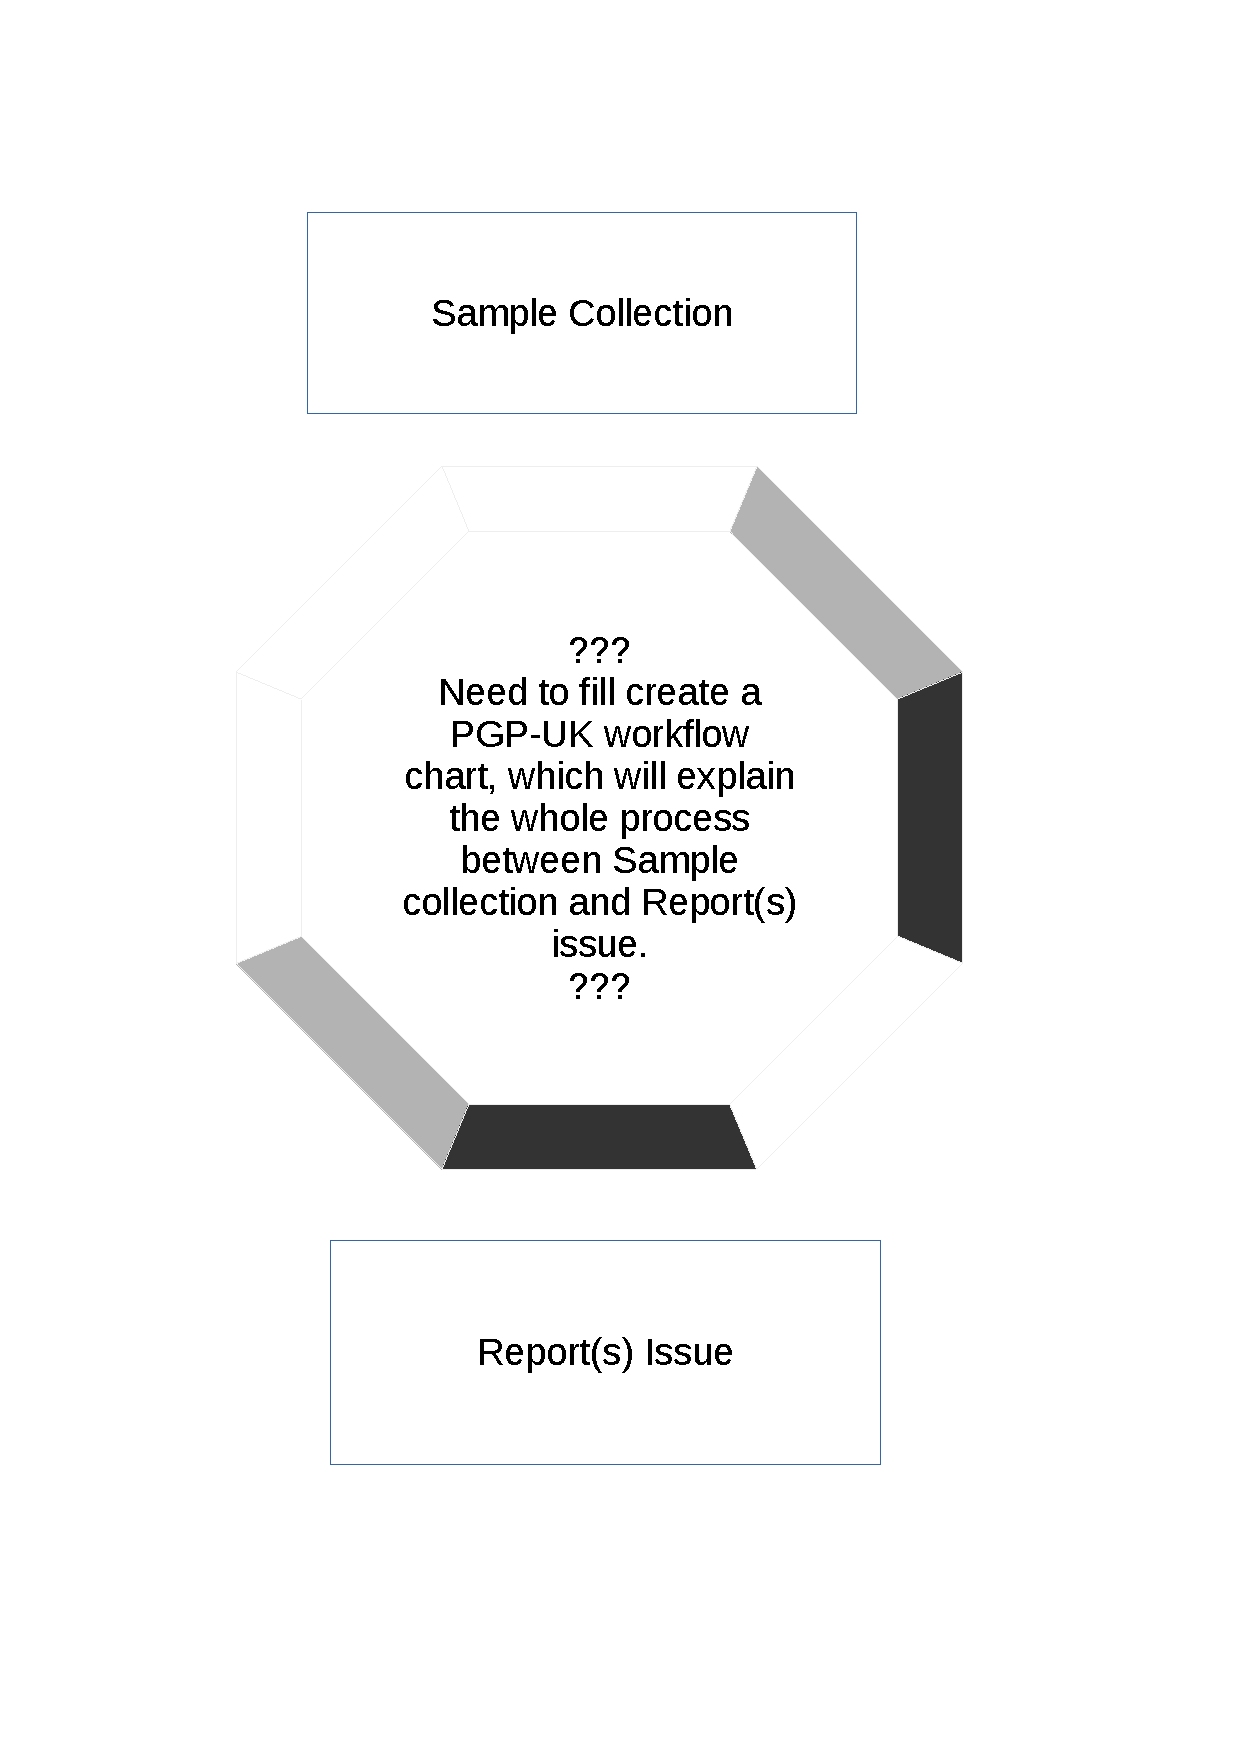
\includegraphics[width = \textwidth]{img/pgpuk.pdf}
\caption{PGP-UK workflow \newline
\textbf{??? Need to be re-done}}
\label{fig: PGP-UK workflow}
\end{figure}


\begin{figure}
    \centering
    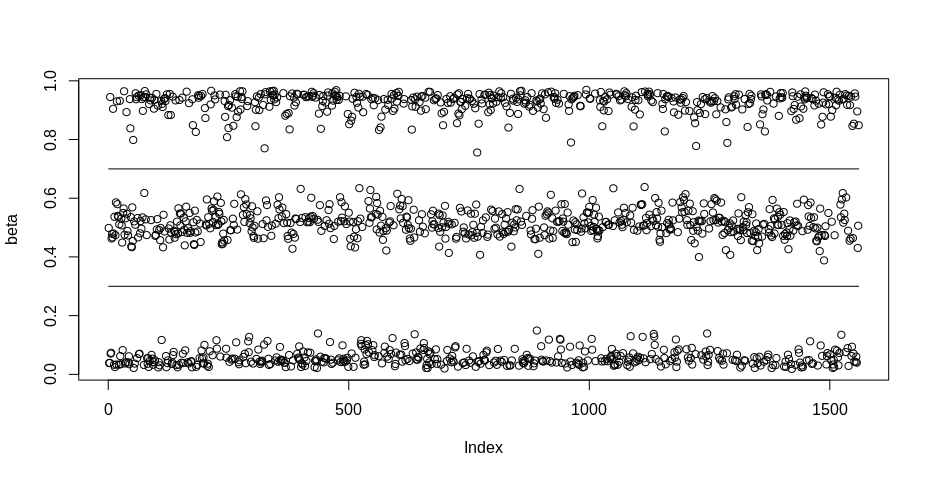
\includegraphics[width=\textwidth]{img/beta_snp65.png}
    \caption{$\beta$-values distribution for Illumina 450k control probes. Horizontal lines represent $\beta=0.3$ and $\beta=0.7$}
    \label{fig: beta-values distribution for Illumina 450k control probes}
\end{figure}
\begin{figure}
    \centering
    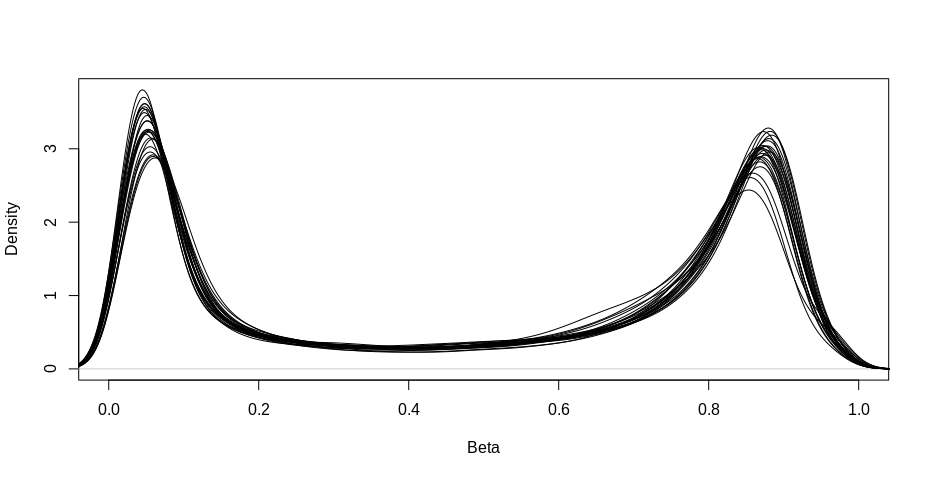
\includegraphics[width=\textwidth]{img/densityPlot450k.png}
    \caption{Density plot for Illumina 450k methylation profiles}
    \label{fig: Density plot for Illumina 450k methylation profiles}
\end{figure}


\section*{Tables}

\textit{Tables supporting the Data Descriptor. These can provide summary information
(sample numbers, demographics, etc.), but they should generally not
be used to present primary data (i.e. measurements). Tables containing
primary data should be submitted to an appropriate data repository. 
\\
Tables may be provided within the \LaTeX{} document or as separate
files (tab-delimited text or Excel files). Legends, where needed,
should be included here. Generally, a Data Descriptor should have
fewer than ten Tables, but more may be allowed when needed. Tables
may be of any size, but only Tables which fit onto a single printed
page will be included in the PDF version of the article (up to a maximum
of three).}

\begin{table}[htb]
\begin{tabular}{|l|c|c|c|c|c|c|}
\hline
 &  & \multicolumn{2}{|c|}{Number of Samples} & \multirow{2}{*}{File Format(s)} & \multirow{2}{*}{Repository} & \multirow{2}{*}{Accession Number} \\ 
 \cline{3-4}
 & & blood & saliva & & & \\
 \hline
\multirow{3}{*}{Genome} & WGS &   &  & \multirow{3}{*}{\begin{tabular}[c]{@{}c@{}}FASTQ\\ BAM\\ VCF\end{tabular}} & \multirow{2}{*}{} & \multirow{2}{*}{} \\ 
\cline{2-4}
\cline{6-7}
 & WXS &  &  &  &  &  \\ 
 \cline{2-4} \cline{6-7} 
 & WGBS &   &  &  &  &  \\ 
 \hline
\multirow{2}{*}{Methylome} & 450k &   &  & \multirow{2}{*}{IDAT} & \multirow{2}{*}{ArrayExpress} & \multirow{2}{*}{}\\ 
\cline{2-4}
 & EPIC &  &  &  &  &  \\ 
 \hline
\multirow{2}{*}{Transcriptome} & \begin{tabular}[c]{@{}c@{}}Whole\\ RNA-Seq\end{tabular} &  &  & FASTQ & \multirow{2}{*}{} & \multirow{2}{*}{} \\ 
\cline{2-5}
 & \begin{tabular}[c]{@{}c@{}}Targeted\\ RNA-Seq\end{tabular} &  &  & \begin{tabular}[c]{@{}c@{}}FASTQ\\ BAM\end{tabular} &  &  \\ 
 \hline
\end{tabular}
\caption{Summary of the PGP-UK data \textbf{Should be edited!}}
\label{tab: Summary of the PGP-UK data}
\end{table}

\begin{table}[]
\centering
%\resizebox{\textwidth}{!}{%
\begin{tabular}{|l|c|c|}
\hline
\hline
\multirow{2}{*}{\textbf{Available Data combination}} & \multicolumn{2}{c|}{\textbf{Number of Samples}} \\
\cline{2-3}
& \textbf{blood} & \textbf{saliva} \\
\hline
\hline
450k \& WXS & 2 & 0\\ \hline
450k \& WGS & 1 & 1\\ 
\hline
450k, WGS, WGBS \& RNA-seq & 10 & 10\\ 
\hline
\hline
EPIC \& WGS & \textbf{90???} & \textbf{0???}\\ 
\hline
\hline
\end{tabular}%
%}
\caption{Data sets combinations available for the PGP-UK participants}
\label{tab: Data sets available for the PGP-UK participants}
\end{table}






\begin{thebibliography}{1}
\expandafter\ifx\csname url\endcsname\relax
  \def\url#1{\texttt{#1}}\fi
\expandafter\ifx\csname urlprefix\endcsname\relax\def\urlprefix{URL }\fi
\providecommand{\bibinfo}[2]{#2}
\providecommand{\eprint}[2][]{\url{#2}}

\bibitem{1000genomes}
  \bibinfo{author}{1000 Genomes Project Consortium}  \emph{et~al.}
    \newblock \bibinfo{title}{{A global reference for human genetic variation}}.
  \newblock \emph{\bibinfo{journal}{Nature}}
  \textbf{\bibinfo{volume}{526}},
  \bibinfo{number}{7571},
  \bibinfo{pages}{68}
  (\bibinfo{year}{2015}).

\bibitem{ancestry}
  \bibinfo{author}{Alexander, D.H.}, \bibinfo{Novembre, J.} \& \bibinfo{Lange, K.}
    \newblock \bibinfo{title}{{Fast model-based estimation of ancestry in unrelated individuals}}.
  \newblock \emph{\bibinfo{journal}{Genome Research}}
  (\bibinfo{year}{2009}).

\bibitem{minfi}
    \bibinfo{author}{Aryee, M.J.} \emph{et~al.}
    \newblock \bibinfo{title}{{Minfi: a flexible and comprehensive Bioconductor package for the analysis of Infinium DNA methylation microarrays}}.
  \newblock \emph{\bibinfo{journal}{Bioinformatics}}
  \textbf{\bibinfo{volume}{30}},
  \bibinfo{number}{10},
  \bibinfo{pages}{1363--1369}
  (\bibinfo{year}{2014}).
  
\bibitem{get_evidence}
  \bibinfo{author}{Ball, M.P.} \emph{et~al.}
    \newblock \bibinfo{title}{{A public resource facilitating clinical use of genomes}}.
  \newblock \emph{\bibinfo{journal}{Proceedings of the National Academy of Sciences}}
  \textbf{\bibinfo{volume}{109}},
  \bibinfo{number}{30},
  \bibinfo{pages}{11920--11927}
  (\bibinfo{year}{2012}).
  
\bibitem{pgp10}
  \bibinfo{author}{Beck, S.} \emph{et~al.}
    \newblock \bibinfo{title}{{PGP-UK: a research and citizen science hybrid project in support of personalized medicine}}.
  \newblock \emph{\bibinfo{journal}{bioRxiv}}
  \bibinfo{pages}{288829}
  (\bibinfo{year}{2018}).
  
\bibitem{pgpQA}
  \bibinfo{author}{Beck, S.}
    \newblock \bibinfo{title}{{Getting up close and personal with UK genomics and beyond}}.
  \newblock \emph{\bibinfo{journal}{Genome medicine}}
  \textbf{\bibinfo{volume}{10}},
  \bibinfo{number}{1},
  \bibinfo{pages}{38}
  (\bibinfo{year}{2018}).

\bibitem{snpedia}
    \bibinfo{author}{Cariaso, M.} \&  \bibinfo{author}{Lennon, G.},
      \bibinfo{title}{{SNPedia: a wiki supporting personal genome annotation, interpretation and analysis}}.
    \newblock \emph{\bibinfo{journal}{Nucleic Acids Research}}
    \textbf{\bibinfo{volume}{40}},
    \bibinfo{number}{D1},
    \bibinfo{pages}{D1308--D1312}
    (\bibinfo{year}{2011}).

\bibitem{chen2013discovery}
    \bibinfo{author}{Chen, Yi.} \emph{et~al.}
      \bibinfo{title}{{Discovery of cross-reactive probes and polymorphic CpGs in the Illumina Infinium HumanMethylation450 microarray}}.
    \newblock \emph{\bibinfo{journal}{Epigenetics}}
    \textbf{\bibinfo{volume}{8}},
    \bibinfo{number}{2},
    \bibinfo{pages}{208--209}
    (\bibinfo{year}{2013}).

\bibitem{smoking_score}
  \bibinfo{author}{Elliott, H.R.}  \emph{et~al.}
    \newblock \bibinfo{title}{{Differences in smoking associated DNA methylation patterns in South Asians and Europeans}}.
  \newblock \emph{\bibinfo{journal}{Clinical Epigenetics}}
  \textbf{\bibinfo{volume}{6}},
  \bibinfo{number}{1},
  \bibinfo{pages}{4}
  (\bibinfo{year}{2014}).

\bibitem{horvath}
  \bibinfo{author}{Horvath, S.}
   \newblock\bibinfo{title}{{DNA methylation age of human tissues and cell types}}.
    \newblock \emph{\bibinfo{journal}{Genome Biology}}
  \textbf{\bibinfo{volume}{14}},
  \bibinfo{number}{10},
  \bibinfo{pages}{3156}
  (\bibinfo{year}{2013}).

\bibitem{clinvar}
  \bibinfo{author}{Landrum, M.J.} \emph{et~al.}
    \newblock \bibinfo{title}{{ClinVar: public archive of interpretations of clinically relevant variants}}.
  \newblock \emph{\bibinfo{journal}{Nucleic Acids Research}}
  \textbf{\bibinfo{volume}{44}},
  \bibinfo{number}{D1},
  \bibinfo{pages}{D862--D868}
  (\bibinfo{year}{2015}).

\bibitem{gnomad}
  \bibinfo{author}{Lek, M.} \emph{et~al.}
    \newblock \bibinfo{title}{{Analysis of protein-coding genetic variation in 60,706 humans}}.
  \newblock \emph{\bibinfo{journal}{Nature}}
  \textbf{\bibinfo{volume}{536}},
  \bibinfo{number}{7616},
  \bibinfo{pages}{285}
  (\bibinfo{year}{2016}).

\bibitem{bwa_mem}
  \bibinfo{author}{Li, H.} \& \bibinfo{author}{Durbin, R.},
  \newblock\bibinfo{title}{{Fast and accurate short read alignment with Burrows--Wheeler transform}}.
  \newblock \emph{\bibinfo{journal}{Bioinformatics}}
  \textbf{\bibinfo{volume}{25}},
  \bibinfo{pages}{1754--1760}
  (\bibinfo{year}{2009}).

\bibitem{samtools}
  \bibinfo{author}{Li, H.} \emph{et~al.}
  \newblock\bibinfo{title}{{The sequence alignment/map format and SAMtools}}.
  \newblock \emph{\bibinfo{journal}{Bioinformatics}}
  \textbf{\bibinfo{volume}{25}},
  \bibinfo{pages}{2078--2079}
  (\bibinfo{year}{2009}).

\bibitem{gembs_bioinformatics}
  \bibinfo{author}{Marco-Sola, S.}, \bibinfo{author}{Schuyler, R.}, \bibinfo{author}{Gut, I. G} \& \bibinfo{author}{Heath, S.C.}
  \newblock\bibinfo{title}{{gemBS: high throughput processing for DNA methylation data from bisulfite sequencing}}.
  \newblock \emph{\bibinfo{journal}{Bioinformatics}}
  \textbf{\bibinfo{volume}{1}},
  \bibinfo{pages}{6}
  (\bibinfo{year}{2018}).
  
\bibitem{ensembl}
  \bibinfo{author}{McLaren, W.}  \emph{et~al.}
    \bibinfo{title}{{The ensembl variant effect predictor}}.
  \newblock \emph{\bibinfo{journal}{Genome Biology}}
  \textbf{\bibinfo{volume}{17}},
  \bibinfo{number}{1},
  \bibinfo{pages}{122}
  (\bibinfo{year}{2016}).
  
\bibitem{champ2013}
  \bibinfo{author}{Morris, T.J.}  \emph{et~al.}
  \newblock \bibinfo{title}{{ChAMP: 450k chip analysis methylation pipeline}}.
  \newblock \emph{\bibinfo{journal}{Bioinformatics}}
  \textbf{\bibinfo{volume}{30}},
  \bibinfo{number}{3},
  \bibinfo{pages}{428--430}
  (\bibinfo{year}{2013}).
  
\bibitem{champ2017}
   \bibinfo{author}{Tian, Y.}   \emph{et~al.}
    \newblock \bibinfo{title}{{ChAMP: updated methylation analysis pipeline for Illumina BeadChips}}.
  \newblock \emph{\bibinfo{journal}{Bioinformatics}},
 \textbf{\bibinfo{volume}{33}},
  \bibinfo{number}{24},
  \bibinfo{pages}{3982--3984}
  (\bibinfo{year}{2017}).

\end{thebibliography}

\section*{Data Citations}

Bibliographic information for the data records described in the manuscript.
\\1. \emph{European Nucleotide Archive} PRJEB13150.
\\2. \emph{European Nucleotide Archive} PRJEB17529.
\\3. \emph{European Nucleotide Archive} PRJEB25139.
\\4. \emph{ArrayExpress} E-MTAB-5377. 
\\5. \emph{ArrayExpress} E-MTAB-6523.

%\vspace{15pt}
%\textit{Data Citations Format}:\\
%1. Lastname1, Initial1., Lastname2, Initial2., ...\& LastnameN, InitialN. \emph{Repository name} Dataset accession number or DOI (YYYY).

\end{document}